\section{Planning and control}
How to plan paths and trajectories at actuator or platform level, and how to control the robot to execute them. 

\subsection{Spline planning in 1D}
Cubic splines in 1D are curves in the $t$ parameter that fulfill zero-order and first-order derivative constraints, so they allow to interpolate between two points in a soft way.

Compute the cubic polynomial in $t\in[0,1]$ domain:
\begin{equation}
 x(t) = at^3 + bt^2 + ct + d
\end{equation}
with the following four constraints: 
\begin{align}
 x(0) = & x_0 \\
 x(1) = & x_1 \\
 \dot{x}(0) = & \tau_0 \\
 \dot{x}(1) = & \tau_1 \\
\end{align}
Given that: 
\begin{equation}
 \dot{x}(t) = 3at^2 + 2bt + c
\end{equation}
the system of equations to solve is: 
\begin{align}
 & d = x_0 \\ \label{eq:system_spline_1d_1}
 & a+b+c+d = x_1 \\ \label{eq:system_spline_1d_2}
 & c = \tau_0 \\ \label{eq:system_spline_1d_3}
 & 3a+2b+c = \tau_1 \\ \label{eq:system_spline_1d_4}
\end{align}
Substracting 3 times the equation~\ref{eq:system_spline_1d_2} to the equation~\ref{eq:system_spline_1d_4}, we obtain: 
\begin{equation}
 -b -2c -3d = \tau_1-3x_1; \rightarrow b=3(x_1-x_0) - 2\tau_0 - \tau_1
\end{equation}
and solving for $a$: 
\begin{equation}
 a=2(x_0-x_1) + \tau_0 + \tau_1
\end{equation}
so in matrix form we can write: 
\begin{equation}
x(t) = \left[
 \begin{array}{cccc}
  t^3 & t^2 & t & 1 \\
 \end{array}
 \right]
 \left[
 \begin{array}{cccc}
  2 & -2 & 1 & 1 \\
  -3 & 3 & -2 & -1\\
  0 & 0 & 1 & 0 \\
  1 & 0 & 0 & 0 \\
 \end{array}
 \right]
 \left[
 \begin{array}{c}
  x_0 \\
  x_1\\
  \tau_0 \\
  \tau_1\\
 \end{array}
 \right]
\end{equation}




\subsection{Spline planning in 2D}

\subsection{A* for Global Planning}

\subsection{PID control}

The diagram in figure~\ref{fig:pid} shows the standard situation for a PID controller. 

\begin{figure}[bth!]
  \begin{center}
    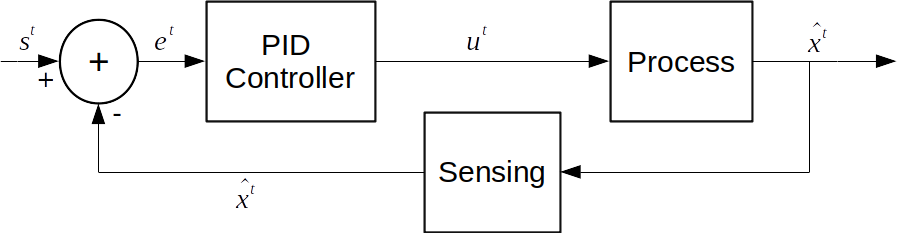
\includegraphics[width=1.0\columnwidth]{figures/pid.png}
    \caption{General diagram for a PID controller.}
    \label{fig:pid}
  \end{center}
\end{figure}


Given a desired, reference or set-point signal~$s^t$, a control command~$u^t$, a process state~$x^t$ and a process state estimate~$\hat{x}^t$ issued from a sensing/perception stage, the error signal is defined as: 
\begin{align}
 & e^t = s^t - \hat{x}^t \\
 & \dot{e}^t = \frac{e^t-e^{t-1}}{\Delta T} \\
 & \bar{e}^t = \sum^N_{j=0} e^{t-j}\Delta T \\
\end{align}
and the output control command is then computed as: 
\begin{equation}
 u^t  = K_p e^t \ + \ K_i \bar{e}^t \ + \ K_d \dot{e}^t
\end{equation}

Algorithm~\ref{alg:pid_controller} summarizes the PID controller using pseudocode related to STL C++ vectors.  
\begin{algorithm}
\caption{PID controller}
\begin{algorithmic}
\STATE WHILE (true)
\STATE \hspace{0.5cm} $s=getSetPoint()$
\STATE \hspace{0.5cm} $x=getSensing()$
\STATE \hspace{0.5cm} $e = s-x$
\STATE \hspace{0.5cm} $ed = (e-ev.back())/\Delta T$
\STATE \hspace{0.5cm} $ev.push\_back(e) = (e-ev.back())/\Delta T$
\STATE \hspace{0.5cm} IF $ev.size()>N$
\STATE \hspace{1cm} $ei = ei+e\Delta T-ev.front()\Delta T $
\STATE \hspace{1cm} $ev.pop\_front()$
\STATE \hspace{0.5cm} ELSE
\STATE \hspace{1cm} $ei = ei+e\Delta T$
\STATE \hspace{0.5cm} END IF
\STATE \hspace{0.5cm} $u = K_p e + K_i ei + K_d ed$
\STATE END WHILE
\end{algorithmic}
\label{alg:pid_controller}
\end{algorithm}

The main difficulty of the PID in practical situations is to correctly tune the constants~$K_p, K_i$ and~$K_d$. The general guidelines for this tunning are, in order: 
\begin{enumerate}
	\item $K_p = K_i = K_d = 0$
	\item Increase $K_p$ up to get some reasonable result.
	\item Reduce the overshoot effect by increasing $K_d$.
	\item Last fine tunning by increasing $K_i$.
\end{enumerate}

The main interpretation of this PID controller is that proportional part is the one mainly driving the control, but the derivative part allows the controller to incorporate some predictive behavior. Finnally the integral contribution gives the possibilty to accurately reach a control reference when the proportional part is near zero.


\subsection{Trajectory control}

\subsection{Dynamical Window Approach (DWA) for wheeled robots}
